\documentclass[11pt,a4paper]{article}
\usepackage[margin=1in]{geometry}
\usepackage{graphicx}
\usepackage{float}
\usepackage{amsmath}
\usepackage{amsfonts}
\usepackage{booktabs}
\usepackage{url}
\usepackage{natbib}
\usepackage{subcaption}
\usepackage{xcolor}
\usepackage{hyperref}

% Color definitions
\definecolor{darkblue}{rgb}{0.0,0.0,0.5}
\hypersetup{
    colorlinks=true,
    linkcolor=darkblue,
    filecolor=darkblue,
    urlcolor=darkblue,
    citecolor=darkblue
}

\title{\Large \textbf{Site Enclosedness \& Fjord Depth Analysis: \\Per-Site Flushing Rates for SSWD-EvoEpi}}

\author{Anton Weerts \\
        OpenClaw Analytics}

\date{\today}

\begin{document}

\maketitle

\begin{abstract}
We present an updated analysis of site enclosedness for the Sea Star Wasting Disease evolutionary epidemiology (SSWD-EvoEpi) study, now incorporating a novel "fjord depth" metric. Using three complementary approaches—tortuosity ratio, horizon exposure ray-casting, and fjord depth—we characterize water exchange potential for 896 sites across 18 regions from Alaska to Baja California. The fjord depth metric, measuring over-water distance to the nearest open-coast site, successfully distinguishes between fjord mouths and fjord heads with similar geometric enclosedness but different connectivity to oceanic water masses. Flushing rates ($\phi$) range from 0.030 to 0.795, with deep fjord sites (SS-S: 259 km depth, JDF: 204 km depth) showing markedly lower flushing than exposed coastal sites (OR: 11 km depth, CA-N: 20 km depth). This refined metric provides crucial spatially-explicit parameters for pathogen transmission models.
\end{abstract}

\tableofcontents
\newpage

\section{Executive Summary}

This report presents a comprehensive three-metric approach for quantifying site enclosedness and water exchange potential in Pacific Northwest marine environments. We analyze 896 sampling sites across 18 biogeographic regions, from Alaskan fjords to Southern California embayments, incorporating:

\begin{itemize}
    \item \textbf{Tortuosity ratio}: Over-water vs.\ straight-line distance based on $k=20$ nearest neighbor connectivity
    \item \textbf{Horizon exposure}: Ray-casting analysis (72 rays, 50 km range) to quantify open-water access
    \item \textbf{Fjord depth}: Over-water distance to nearest open-coast site (enclosedness $< 0.3$)
\end{itemize}

The resulting flushing rates range from $\phi = 0.030$ to $\phi = 0.795$, revealing dramatic differences between deep fjord sites and exposed coastlines. Key findings include exceptional isolation of Puget Sound sites (SS-S: mean depth 259 km) and Strait of Juan de Fuca (JDF: 204 km), contrasted with highly flushed Oregon and Northern California coastal sites.

\section{Methods}

\subsection{Data Overview}

The analysis encompasses 896 marine sampling sites distributed across 18 biogeographic regions spanning approximately 40° of latitude (30°N to 70°N) and 70° of longitude (110°W to 180°W). Sites range from exposed outer-coast locations to deep fjord systems, providing comprehensive coverage of Pacific Northwest marine environments.

\subsection{Tortuosity Ratio}

Tortuosity quantifies the sinuosity of waterways by comparing over-water navigation distances to straight-line (great-circle) distances. For each site, we:

\begin{enumerate}
    \item Identify the $k=20$ nearest neighboring sites
    \item Calculate over-water distances using shortest-path routing around land masses
    \item Calculate corresponding great-circle (haversine) distances
    \item Compute the tortuosity ratio: $T = \frac{\text{over-water distance}}{\text{haversine distance}}$
\end{enumerate}

Values near 1.0 indicate direct water access, while higher values indicate tortuous waterways characteristic of fjord systems.

\subsection{Horizon Exposure Ray-Casting}

Horizon exposure quantifies the fraction of open-water directions from each site using computational ray-casting:

\begin{enumerate}
    \item Cast 72 rays (5° intervals) from each site
    \item Extend rays to 50 km maximum distance
    \item Record intersection with land boundaries
    \item Calculate horizon exposure: $H = \frac{\text{rays reaching 50 km}}{\text{total rays}}$
    \item Compute enclosedness: $E_{\text{rays}} = 1 - H$
\end{enumerate}

This metric captures the geometric "openness" of each site's immediate marine environment.

\subsection{Fjord Depth Metric}

The fjord depth metric measures connectivity to open oceanic water masses by calculating over-water distance to the nearest "open-coast" site. Open-coast sites are defined as those with combined enclosedness $< 0.3$.

\begin{enumerate}
    \item Identify all open-coast reference sites (enclosedness $< 0.3$)
    \item For each target site, calculate over-water distance to all open-coast sites
    \item Record minimum distance as fjord depth: $D_{\text{fjord}}$ (km)
    \item Normalize to [0,1] scale: $D_{\text{norm}} = \min(D_{\text{fjord}}/200, 1)$
\end{enumerate}

This metric distinguishes fjord mouths (low depth, direct oceanic access) from fjord heads (high depth, isolated from oceanic influence).

\subsection{Combined Enclosedness}

Individual metrics are combined into a composite enclosedness measure:

\begin{equation}
E_{\text{combined}} = 0.5 \times \frac{T - 1}{\max(T) - 1} + 0.5 \times E_{\text{rays}}
\end{equation}

where the tortuosity component is normalized to [0,1] scale.

\subsection{Flushing Rate Calculation}

The final flushing rate incorporates both geometric enclosedness and fjord depth:

\begin{align}
E_{\text{effective}} &= E_{\text{combined}} \times (0.5 + 0.5 \times D_{\text{norm}}) \\
\phi &= 0.8 \times (1 - E_{\text{effective}}) + 0.03 \times E_{\text{effective}}
\end{align}

This formulation ensures that:
\begin{itemize}
    \item Fjord mouths receive 50\% of the enclosedness penalty
    \item Fjord heads receive 100\% of the enclosedness penalty
    \item Deep isolation amplifies the effect of geometric enclosedness
\end{itemize}

\section{Results}

\subsection{Spatial Patterns}

Figures~\ref{fig:fjord_depth}--\ref{fig:enclosedness_map} present the spatial distribution of key metrics across the study domain. The fjord depth metric (Figure~\ref{fig:fjord_depth}) reveals striking gradients, with Puget Sound sites reaching depths of 259 km from open ocean, while exposed Oregon and California coastlines maintain depths $< 40$ km.

\begin{figure}[H]
    \centering
    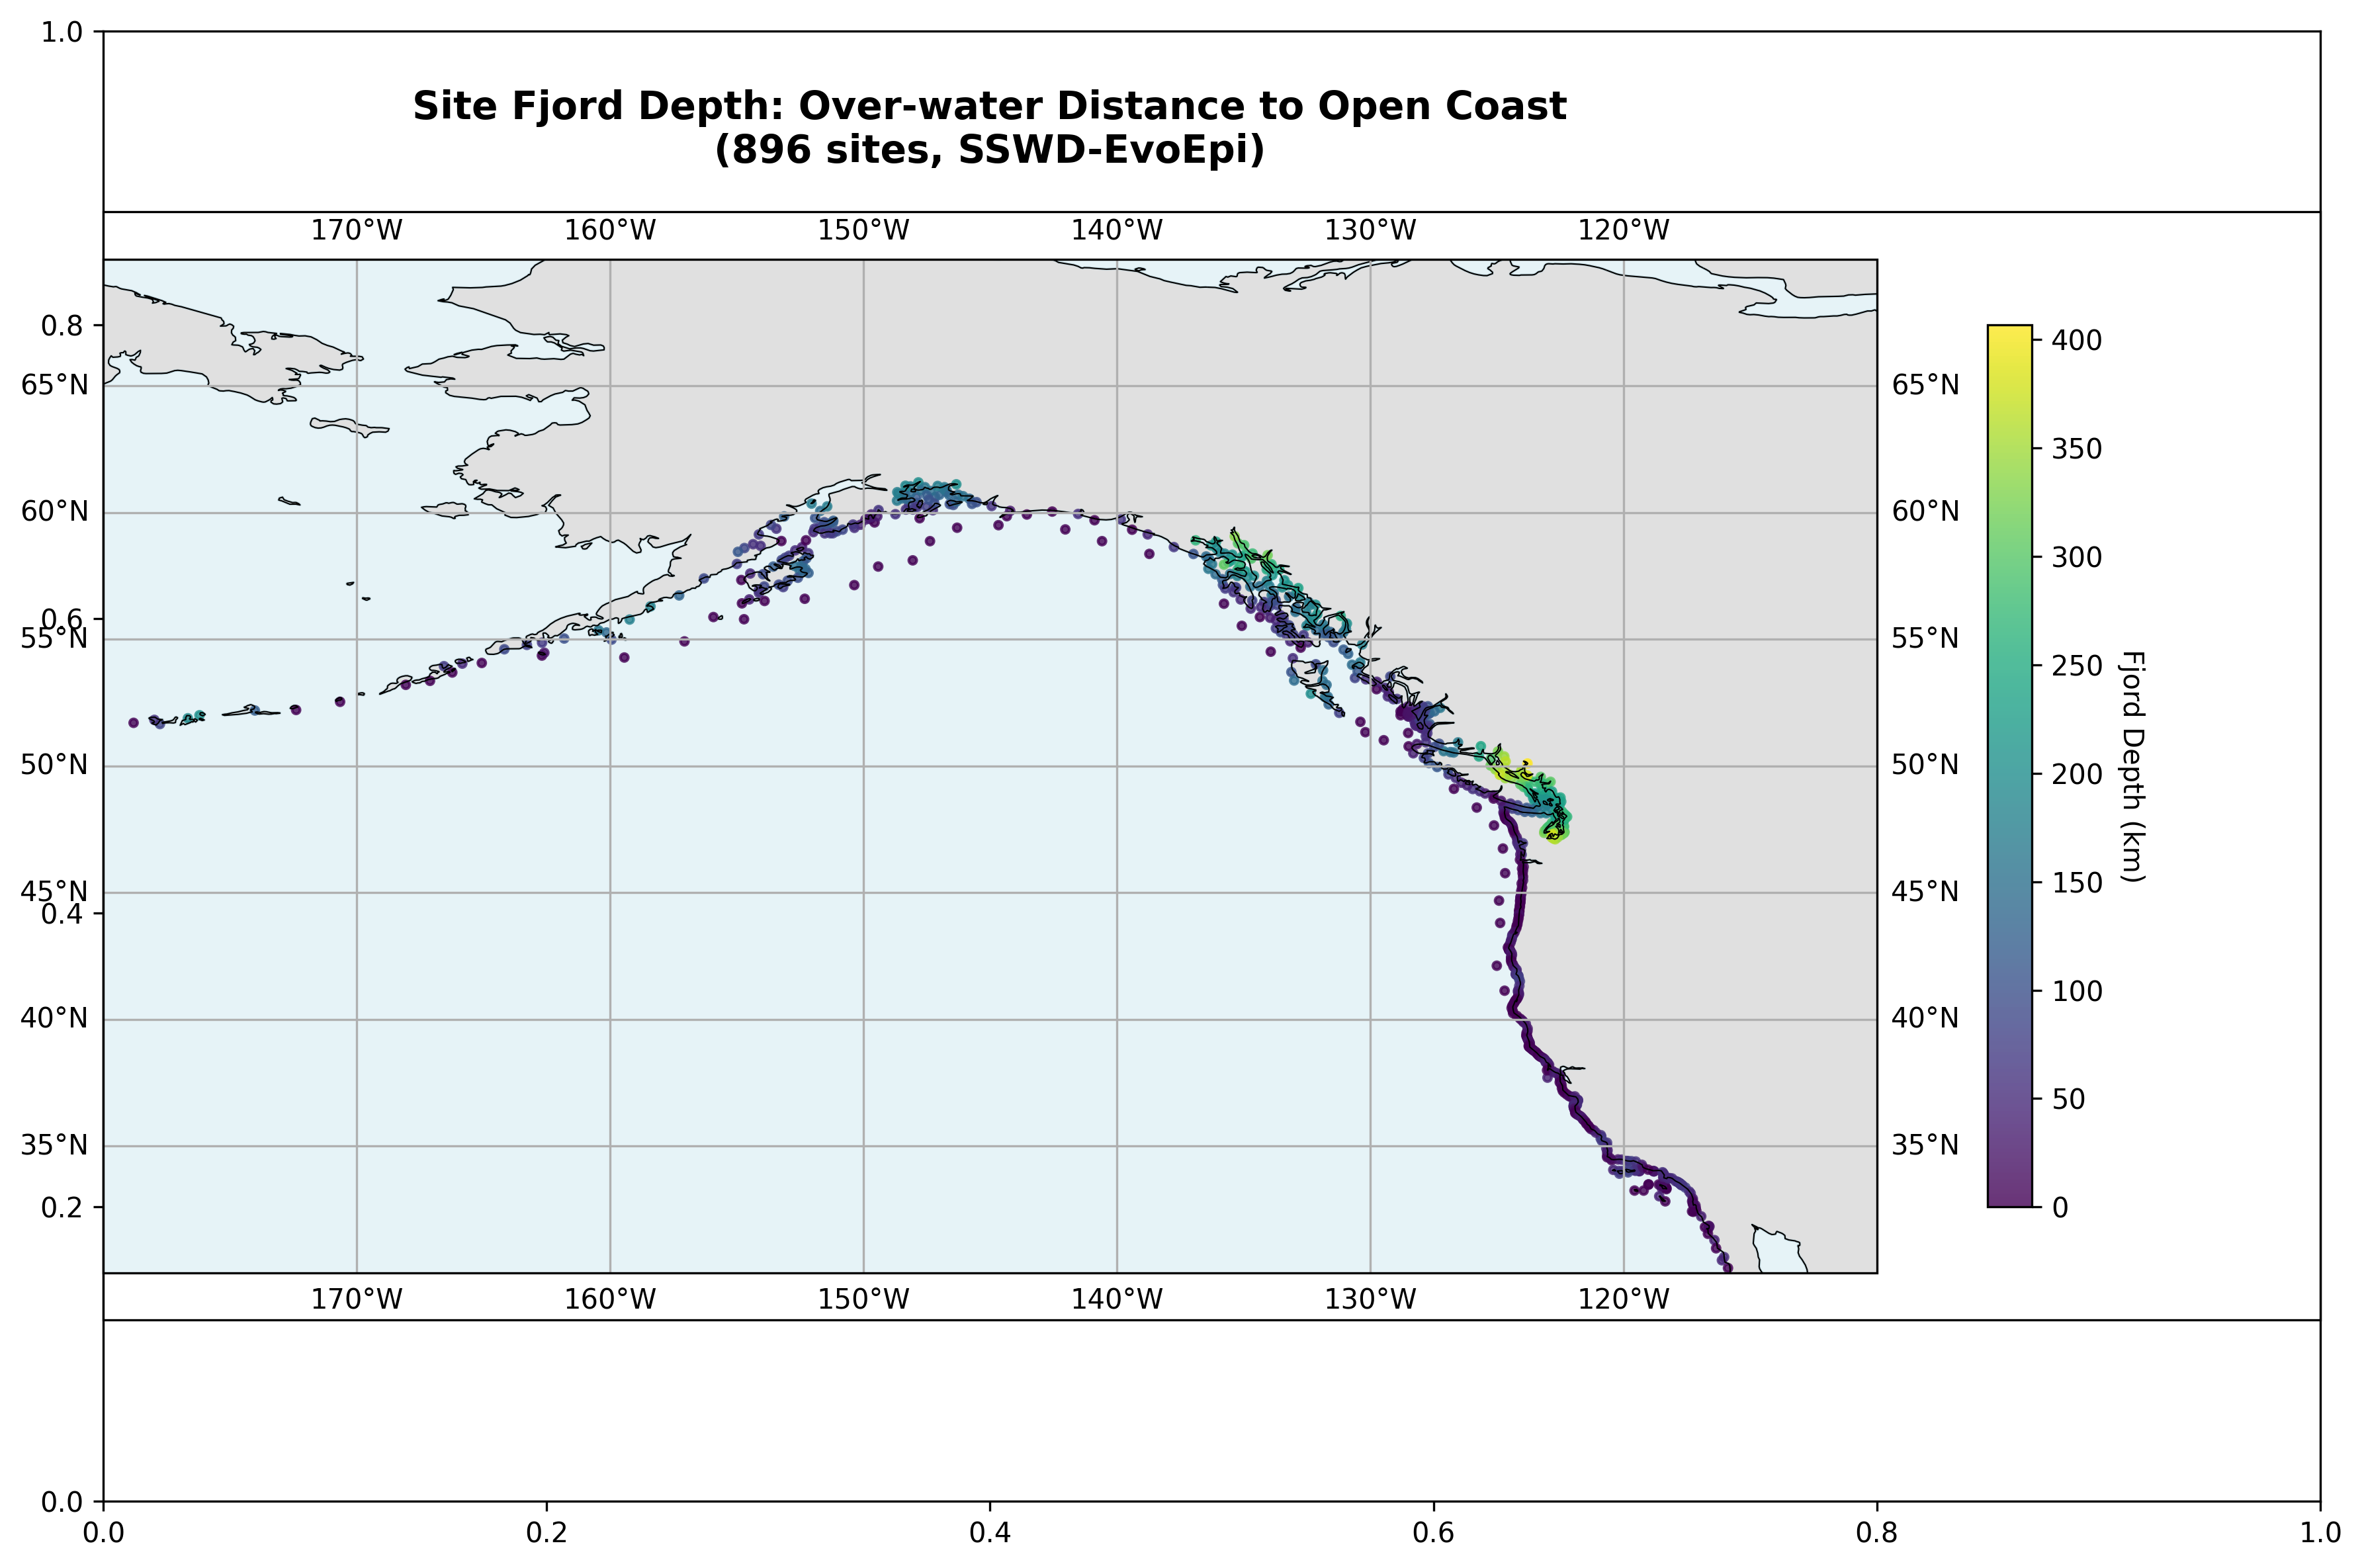
\includegraphics[width=0.95\textwidth]{figures/01_fjord_depth_map.png}
    \caption{Spatial distribution of fjord depth across 896 sampling sites. Fjord depth represents over-water distance (km) to the nearest open-coast site (enclosedness $< 0.3$). Deep purples indicate sites isolated within fjord systems, while yellows represent sites with direct oceanic access.}
    \label{fig:fjord_depth}
\end{figure}

\begin{figure}[H]
    \centering
    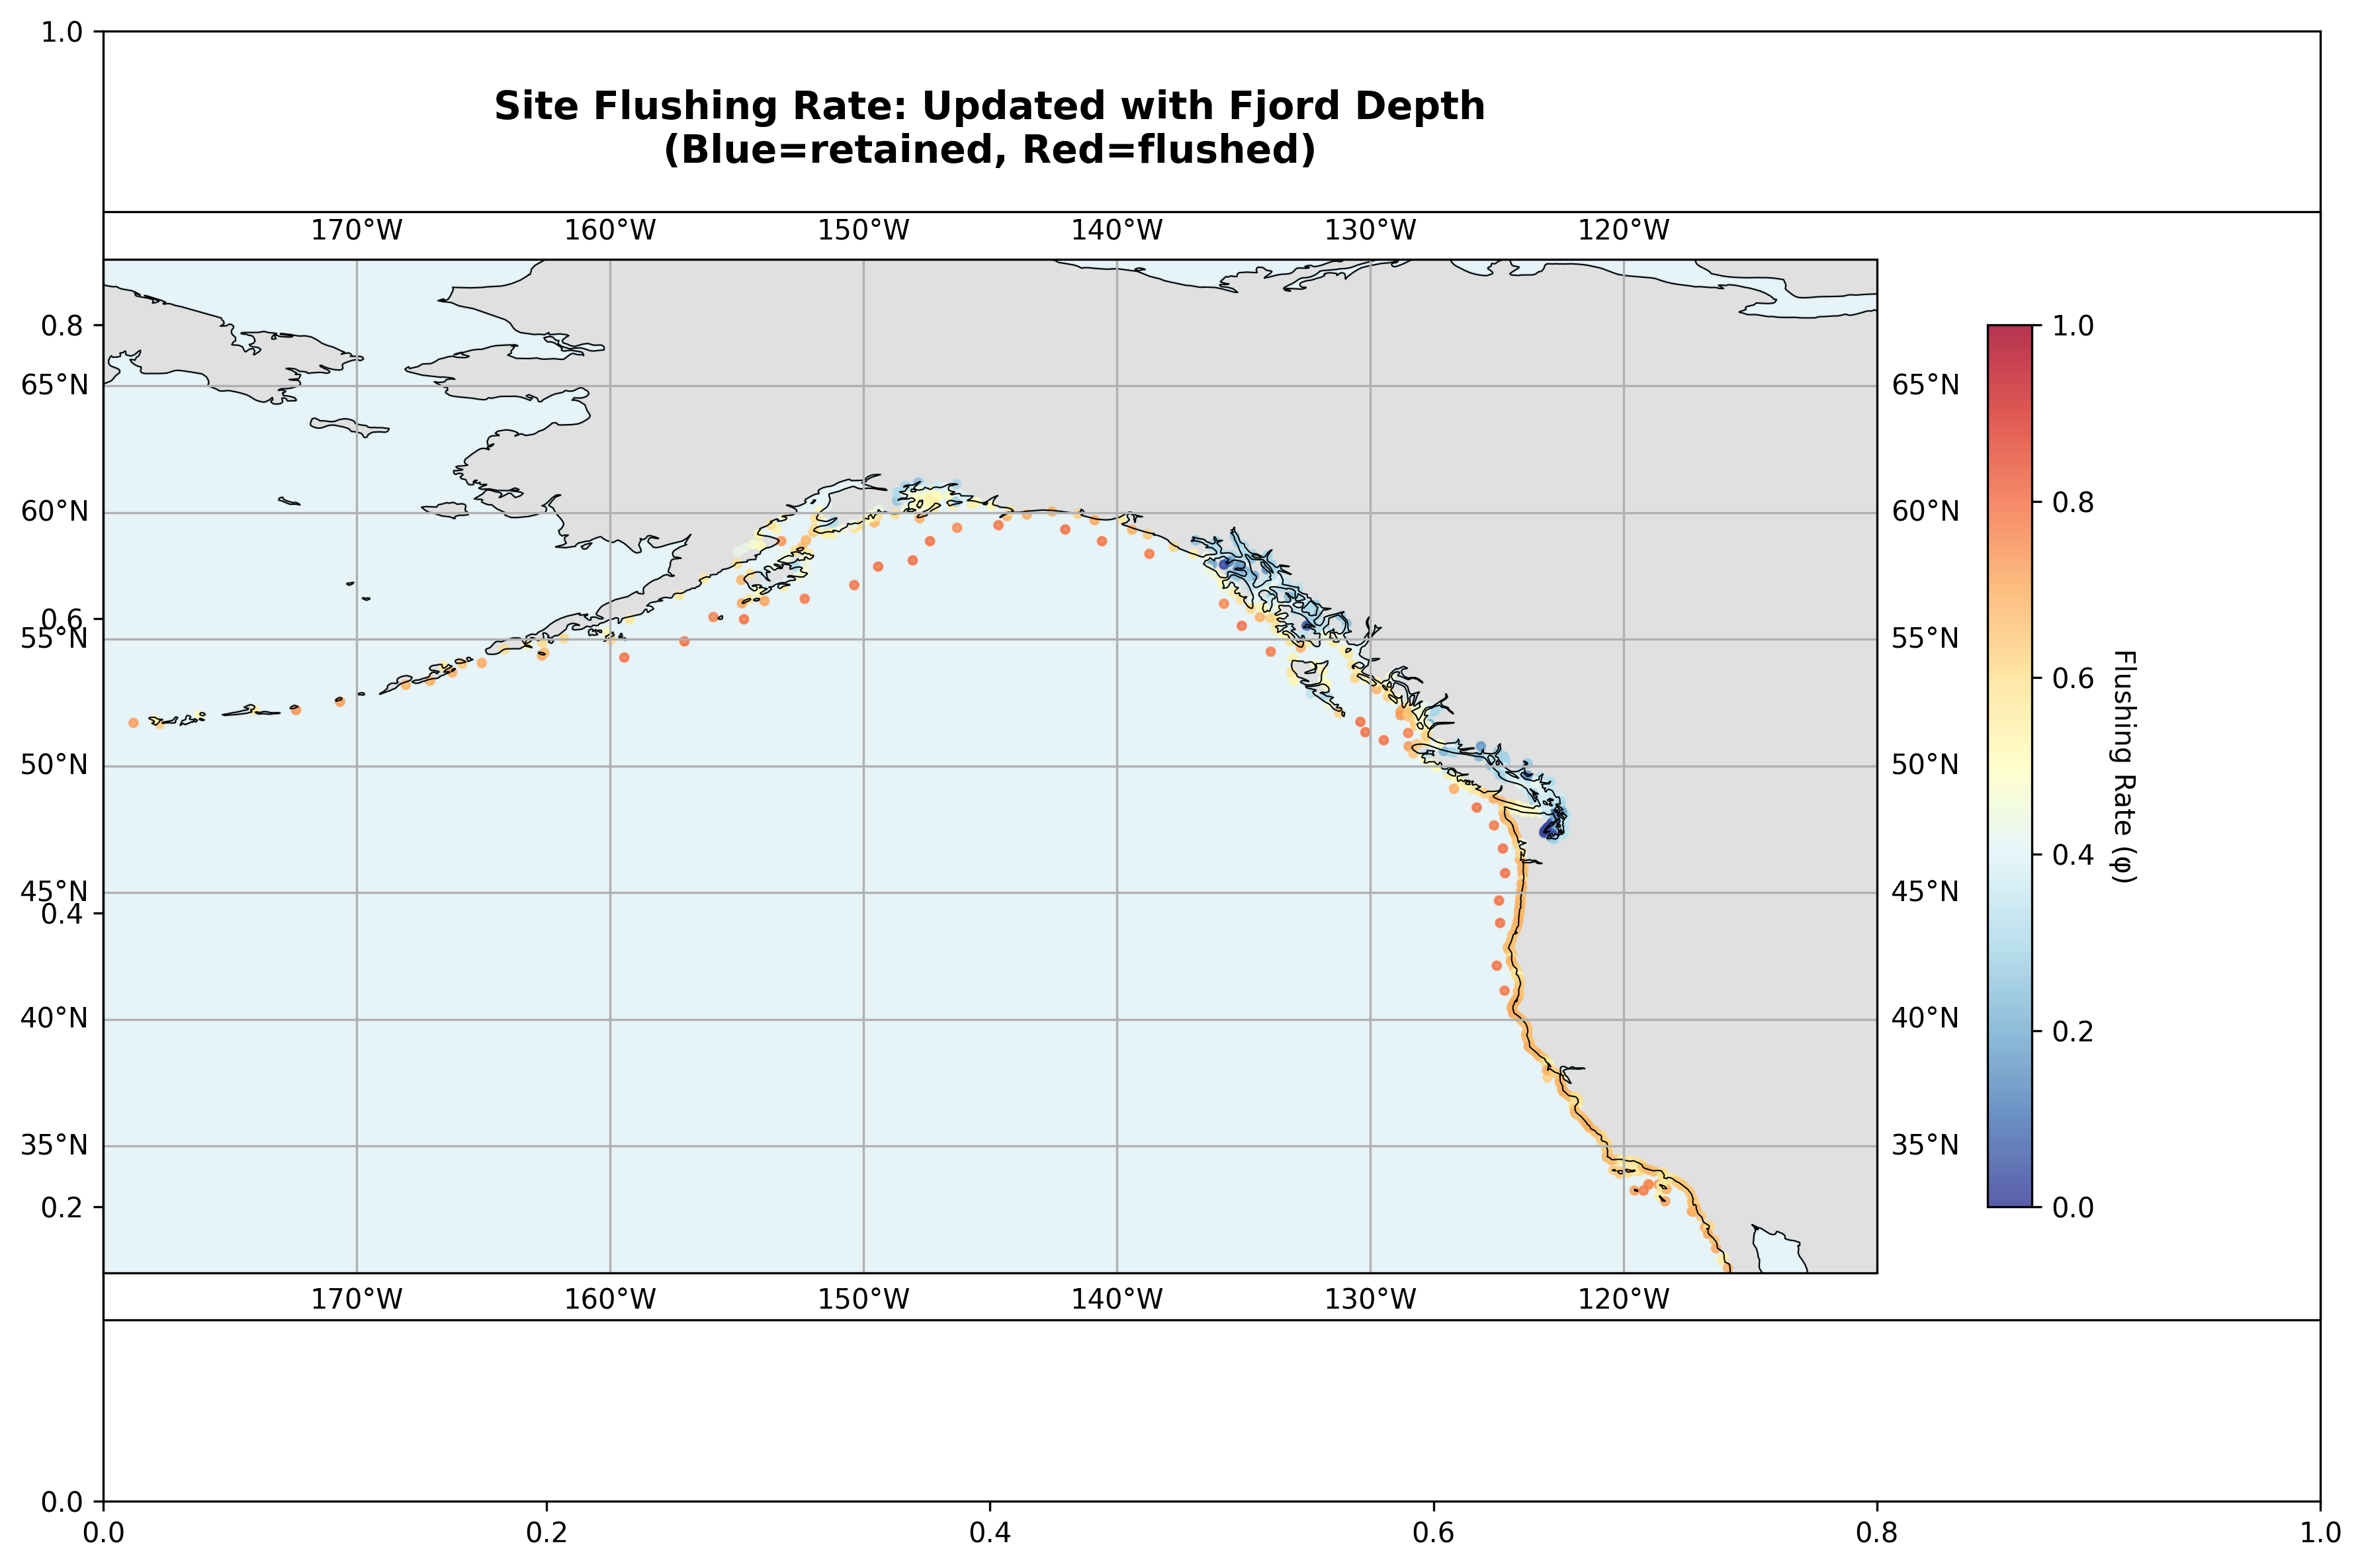
\includegraphics[width=0.95\textwidth]{figures/02_flushing_rate_map.png}
    \caption{Updated flushing rates incorporating fjord depth effects. Blue indicates low flushing (high retention), red indicates high flushing. The fjord depth correction produces more realistic gradients within waterway systems, distinguishing fjord mouths from fjord heads.}
    \label{fig:flushing_map}
\end{figure}

\begin{figure}[H]
    \centering
    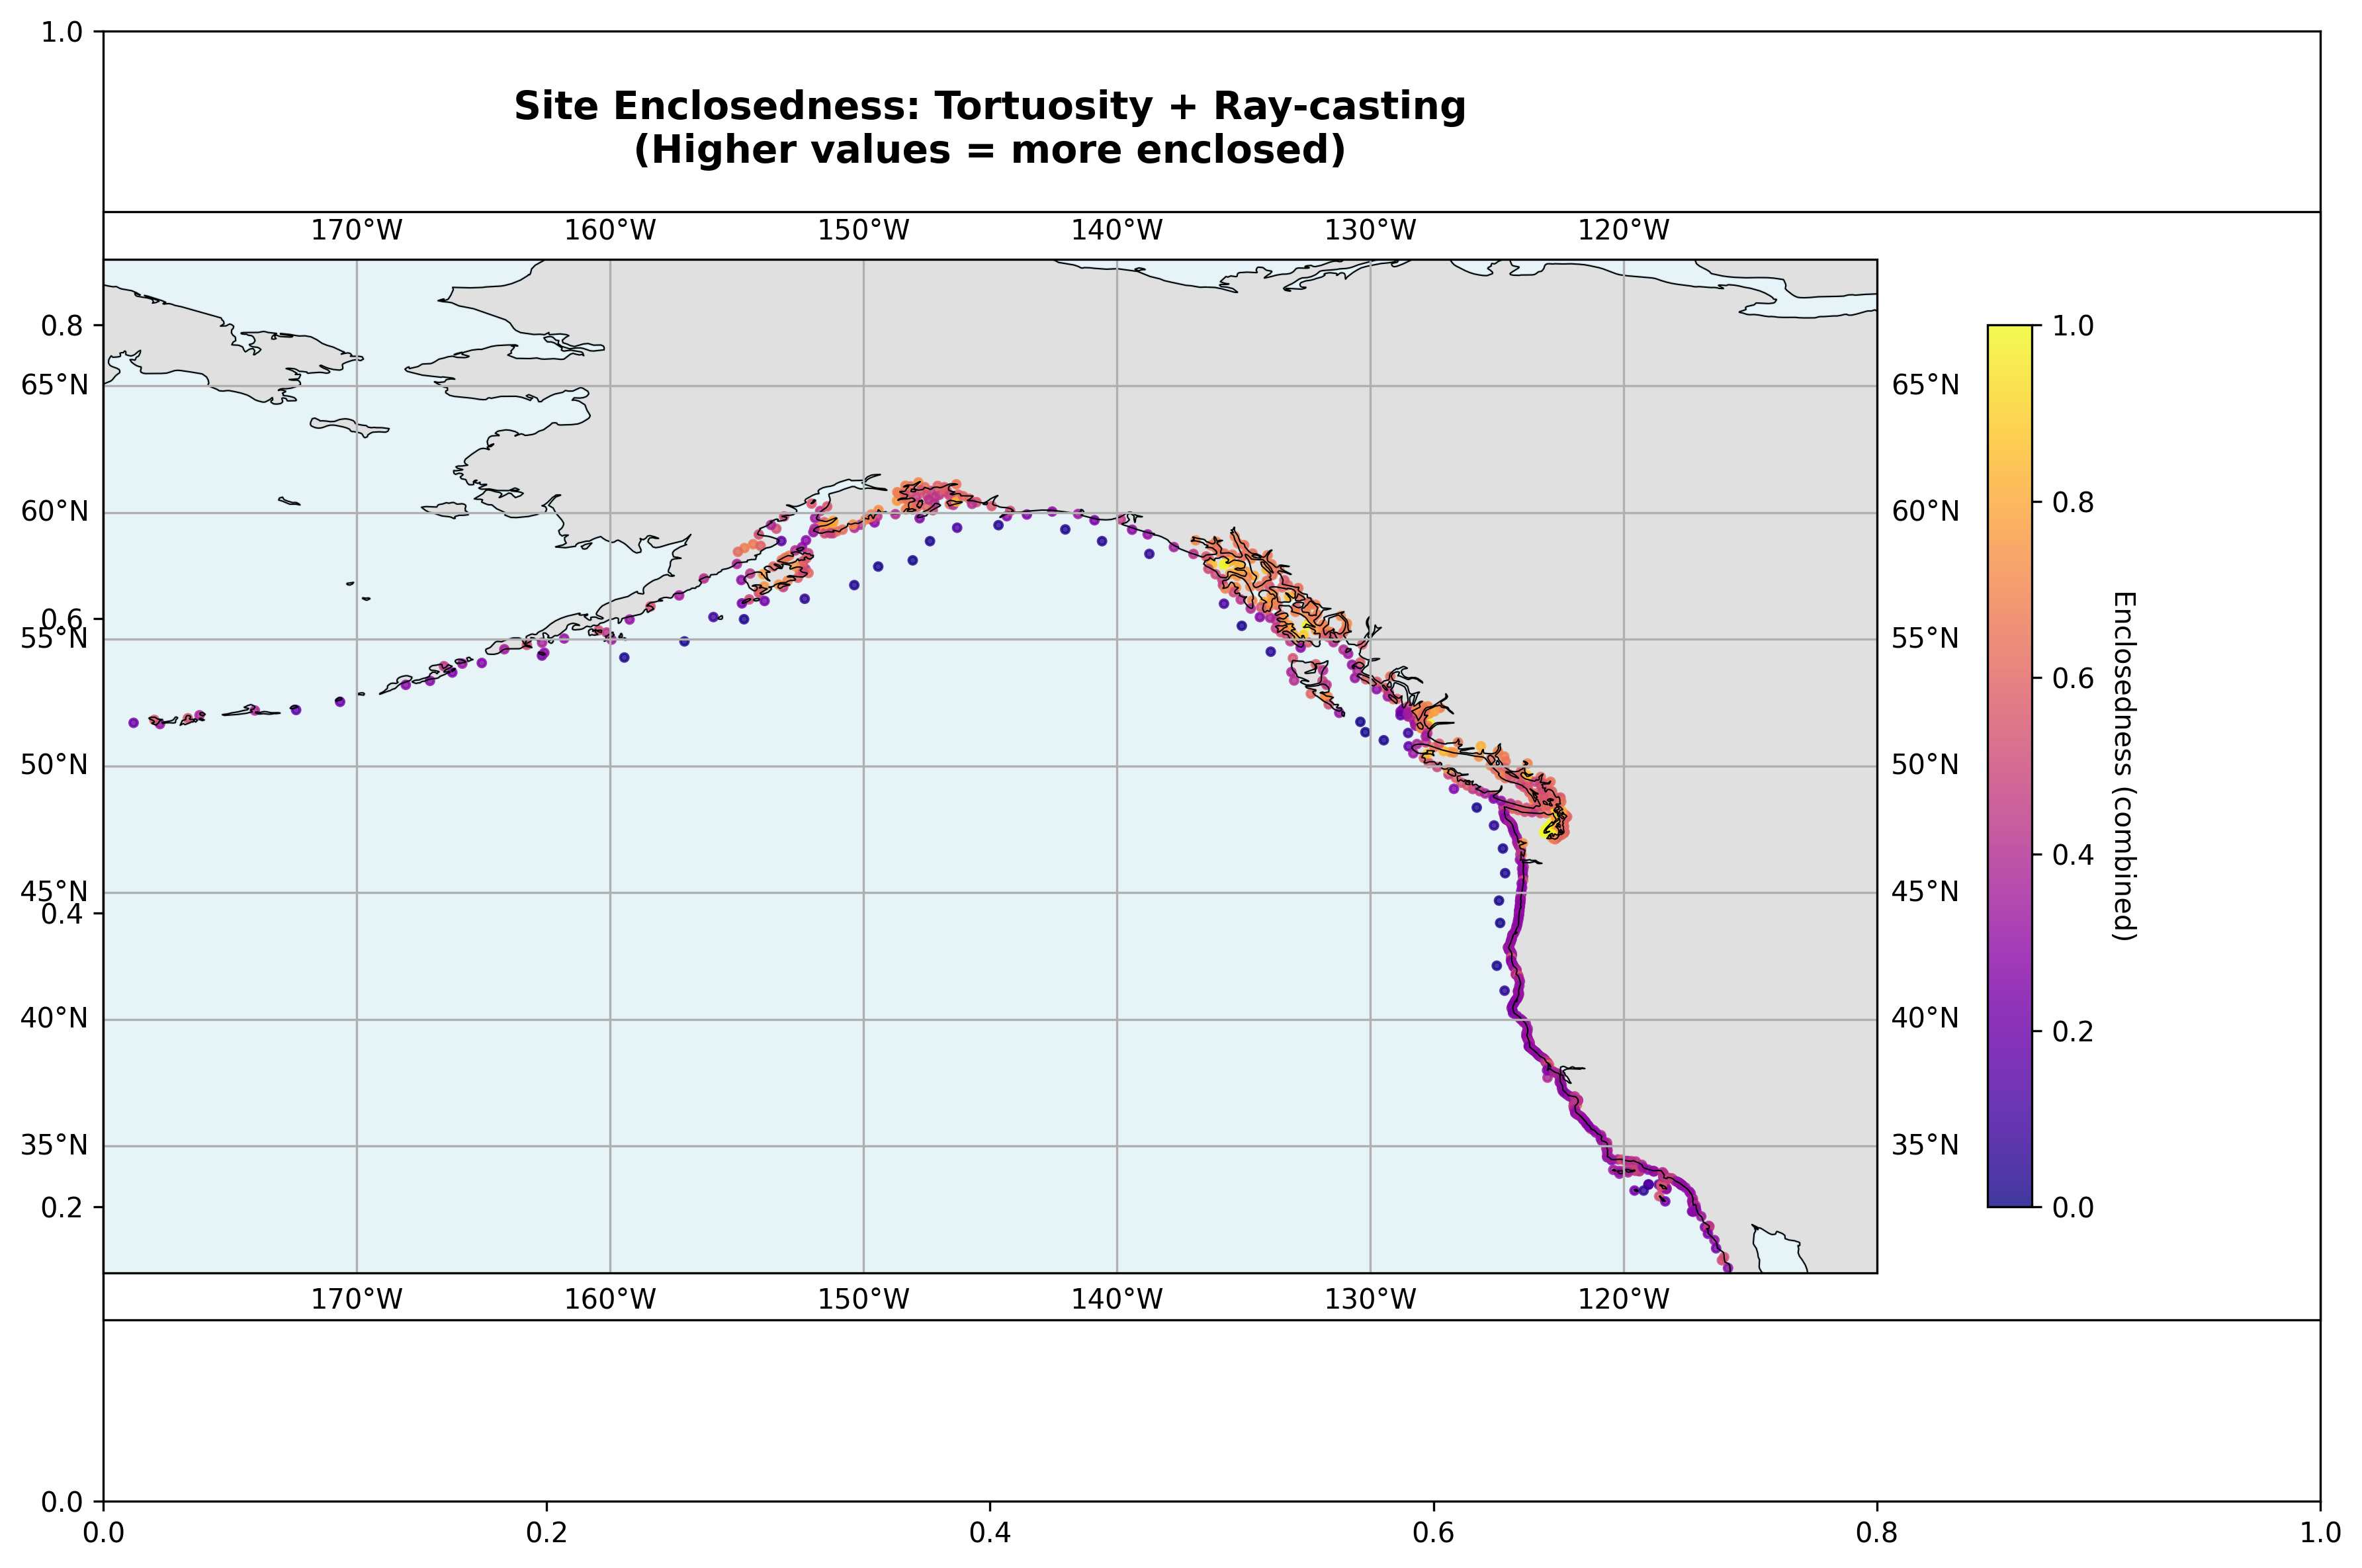
\includegraphics[width=0.95\textwidth]{figures/03_enclosedness_map.png}
    \caption{Combined enclosedness metric incorporating both tortuosity ratio and horizon exposure ray-casting. Higher values (warmer colors) indicate more geometrically enclosed environments.}
    \label{fig:enclosedness_map}
\end{figure}

\subsection{Enclosedness-Depth Relationships}

Figure~\ref{fig:depth_enclosedness} demonstrates the relationship between geometric enclosedness and fjord depth across regions. The scatter reveals distinct clustering patterns:

\begin{itemize}
    \item \textbf{Deep fjords} (high enclosedness + high depth): AK-FN, SS-S, JDF
    \item \textbf{Shallow embayments} (high enclosedness + low depth): BC regions, WA-PS
    \item \textbf{Exposed coasts} (low enclosedness + low depth): OR, CA-N, CA-S
\end{itemize}

\begin{figure}[H]
    \centering
    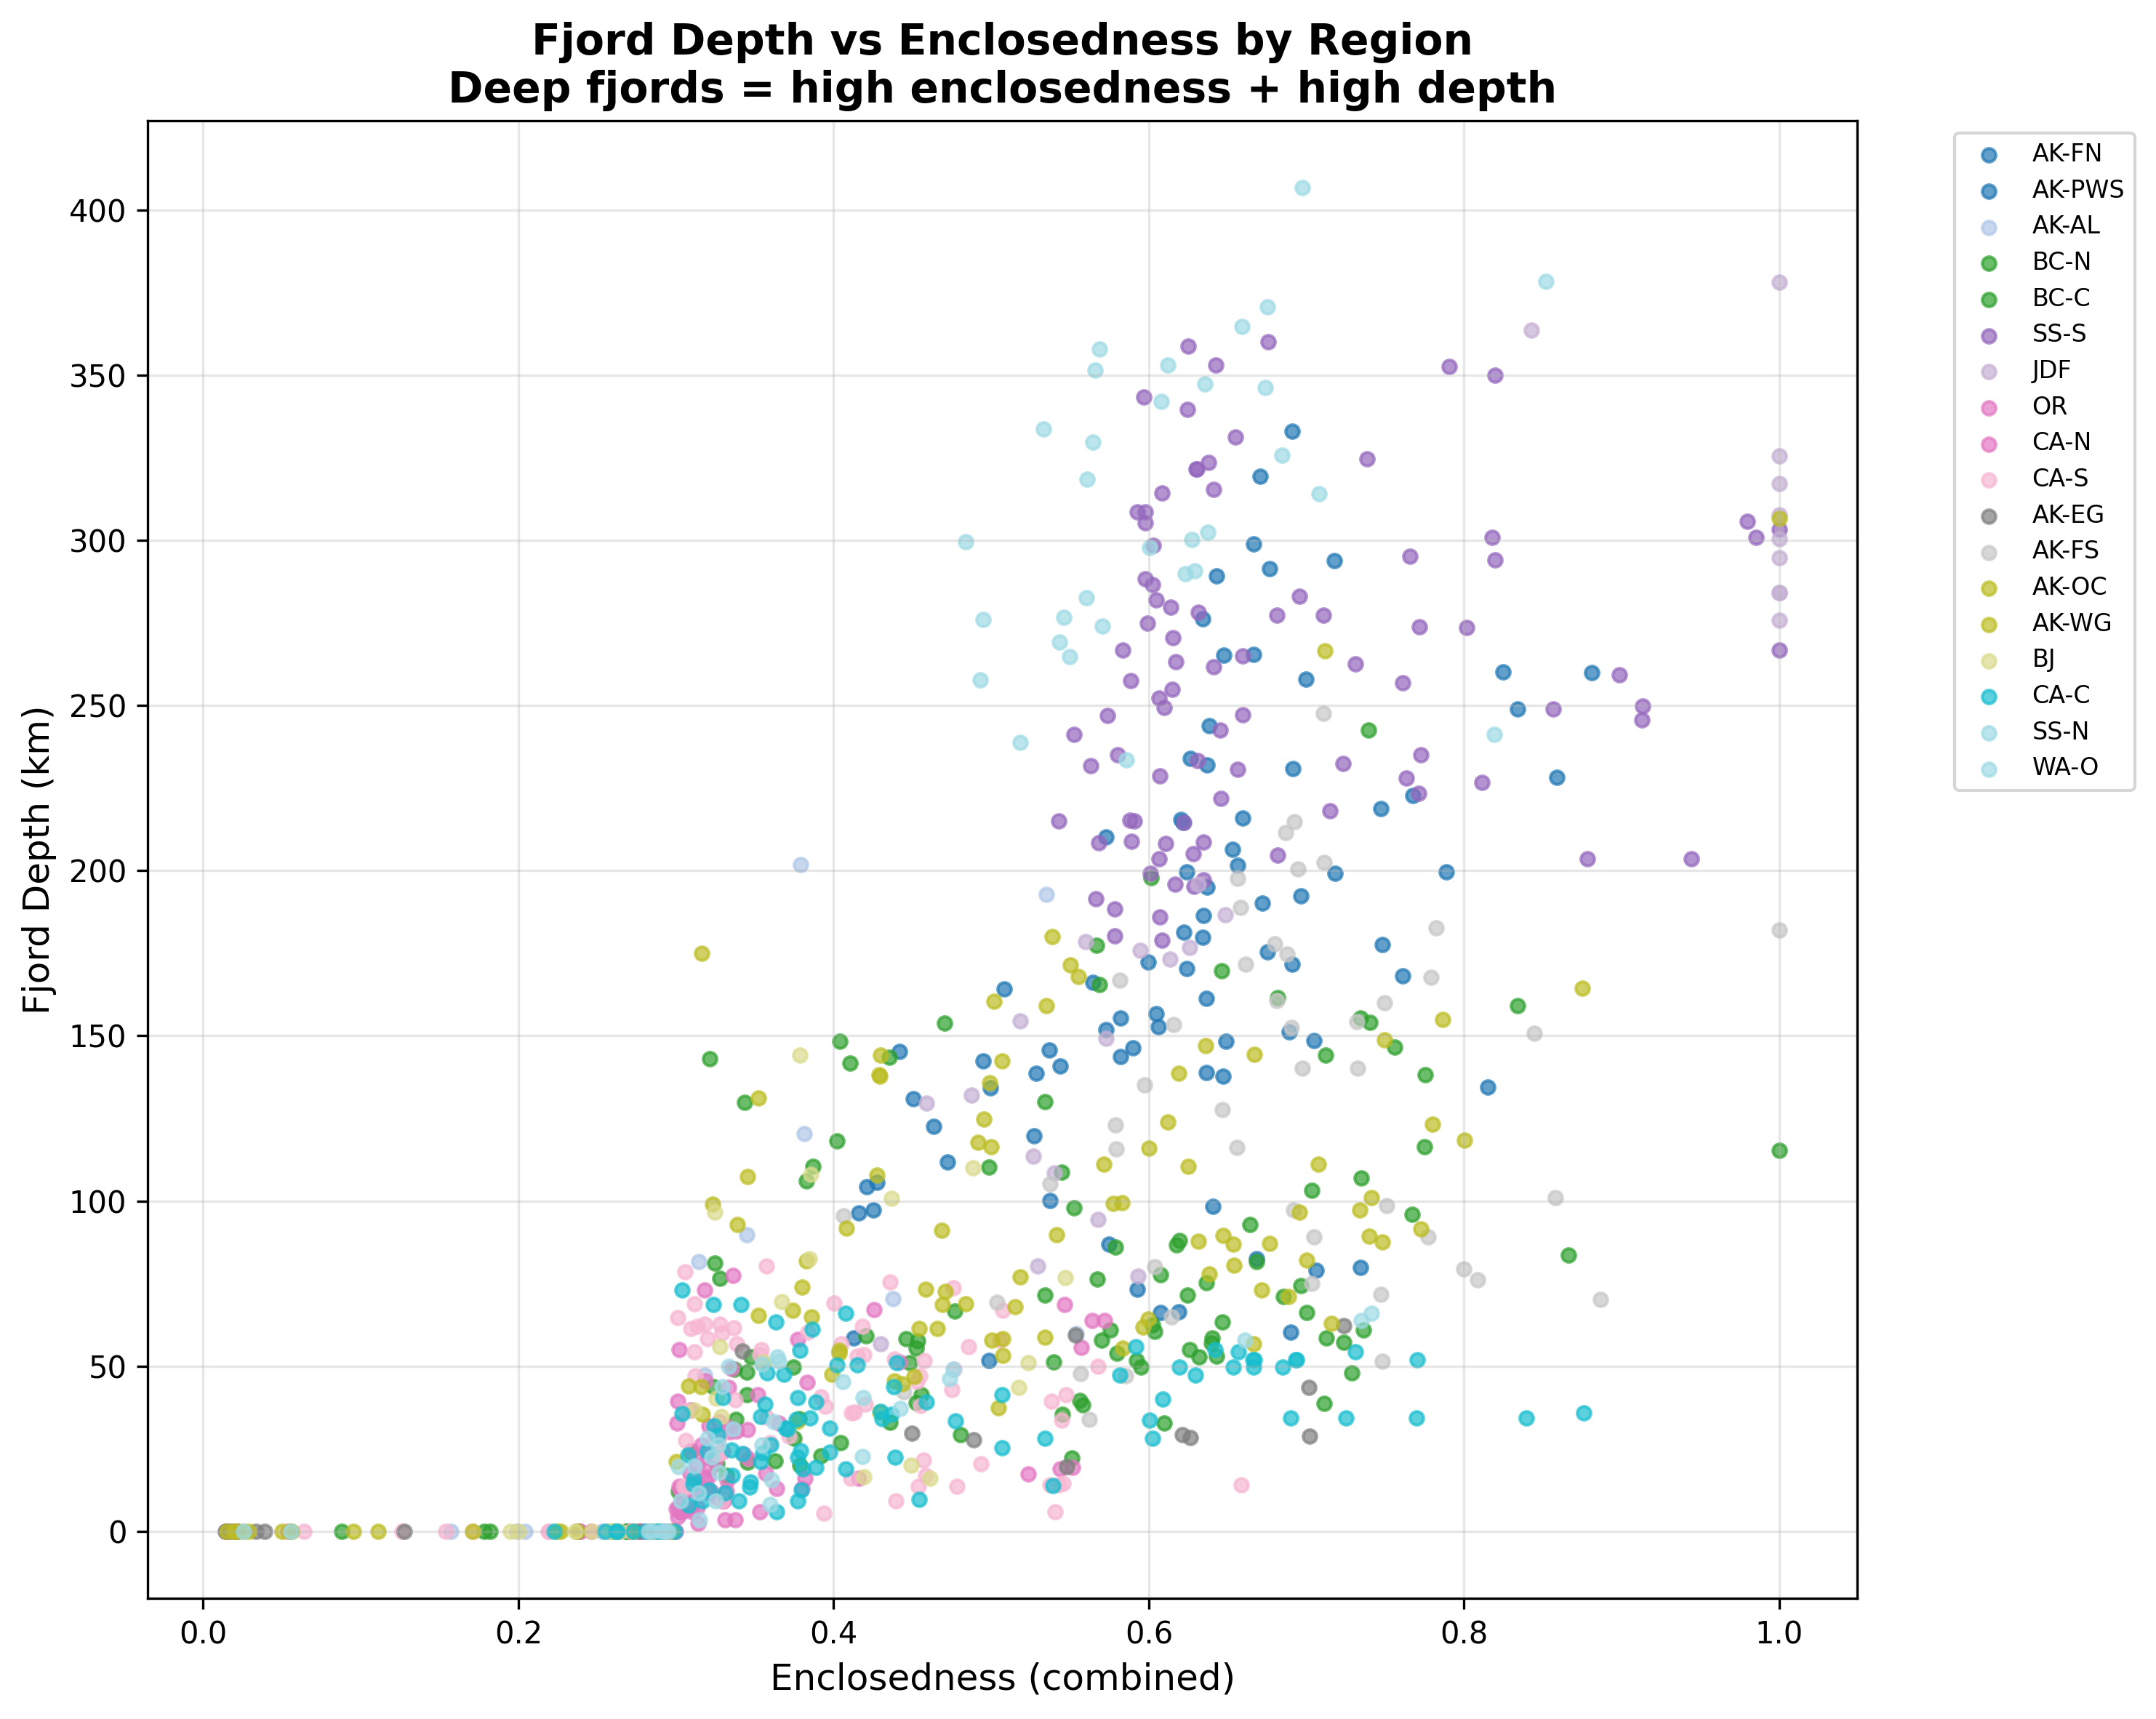
\includegraphics[width=0.9\textwidth]{figures/04_depth_vs_enclosedness.png}
    \caption{Relationship between geometric enclosedness and fjord depth by region. Points in the upper-right quadrant represent deep fjord sites with both high geometric enclosedness and isolation from oceanic water masses. Color coding distinguishes biogeographic regions.}
    \label{fig:depth_enclosedness}
\end{figure}

\subsection{Regional Patterns}

Figures~\ref{fig:flushing_regions} and \ref{fig:depth_regions} reveal systematic latitudinal and physiographic patterns in flushing and fjord depth. Northern regions (Alaska, British Columbia) show greater variability, reflecting complex fjord topography, while southern regions (Oregon, California) show consistently high flushing rates.

\begin{figure}[H]
    \centering
    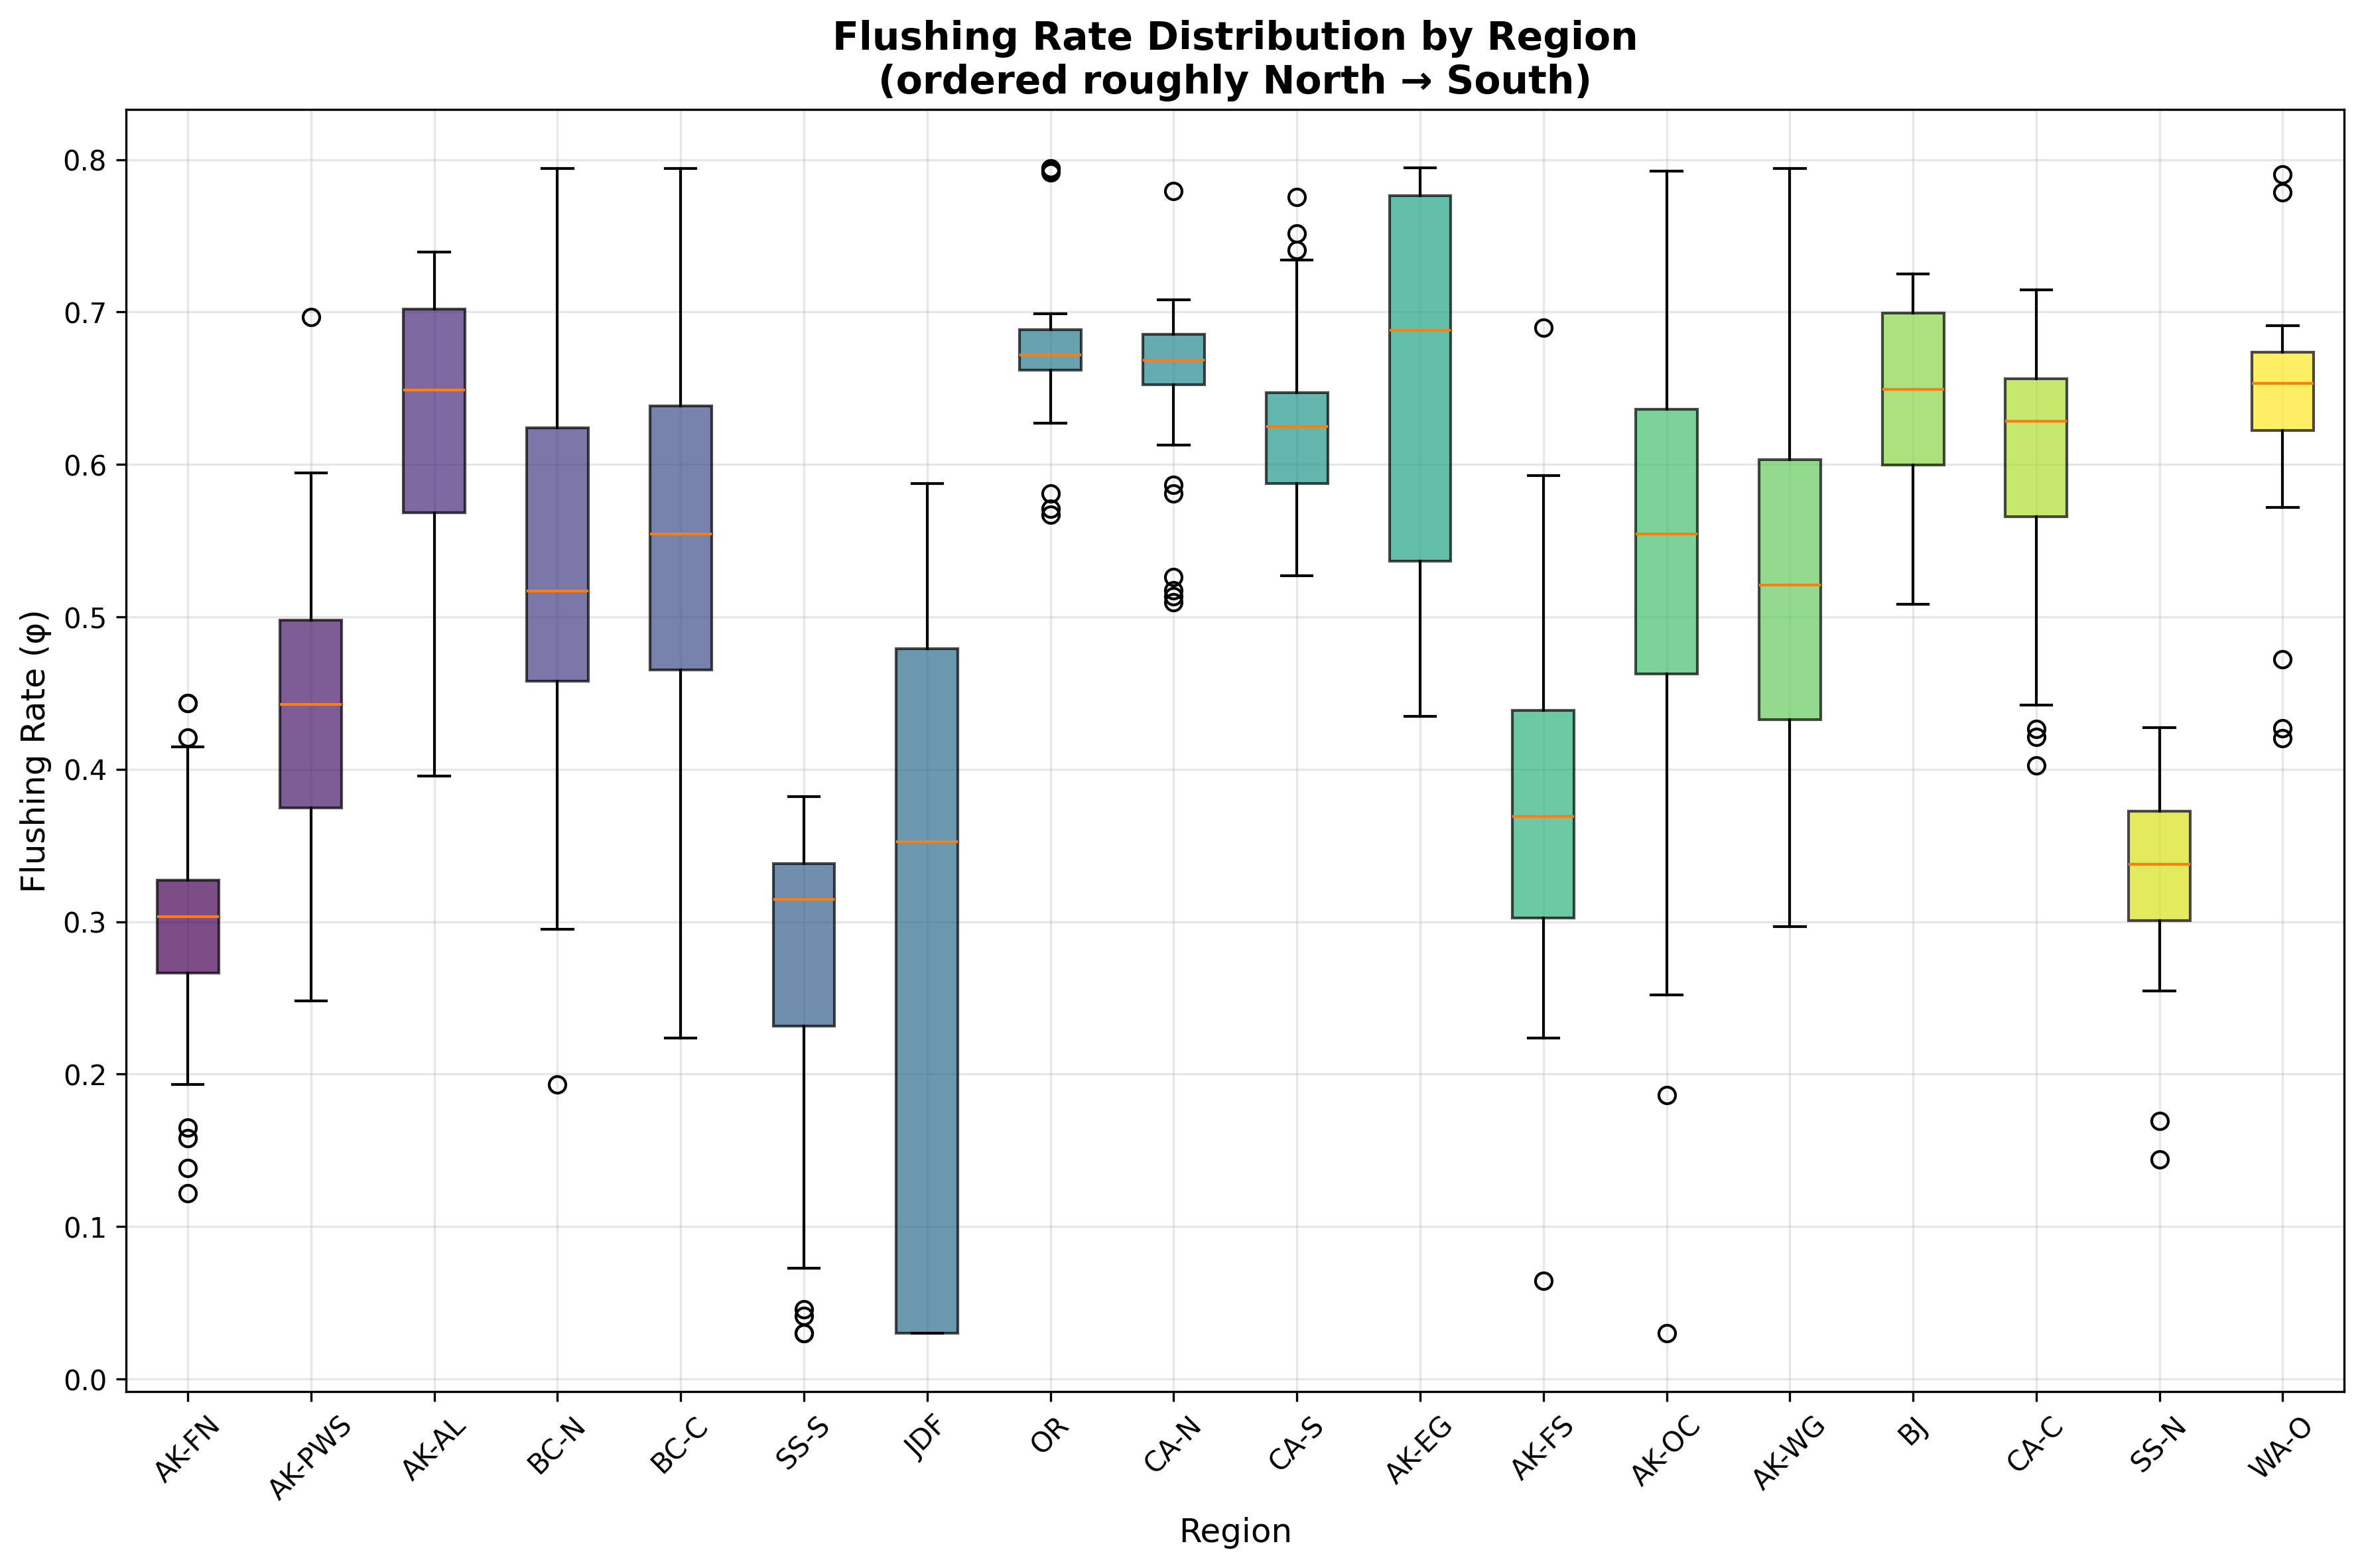
\includegraphics[width=0.95\textwidth]{figures/05_flushing_by_region.png}
    \caption{Distribution of flushing rates by biogeographic region, ordered approximately north to south. Box plots show median (orange line), interquartile range (box), and outliers. Northern fjord regions show consistently lower flushing rates.}
    \label{fig:flushing_regions}
\end{figure}

\begin{figure}[H]
    \centering
    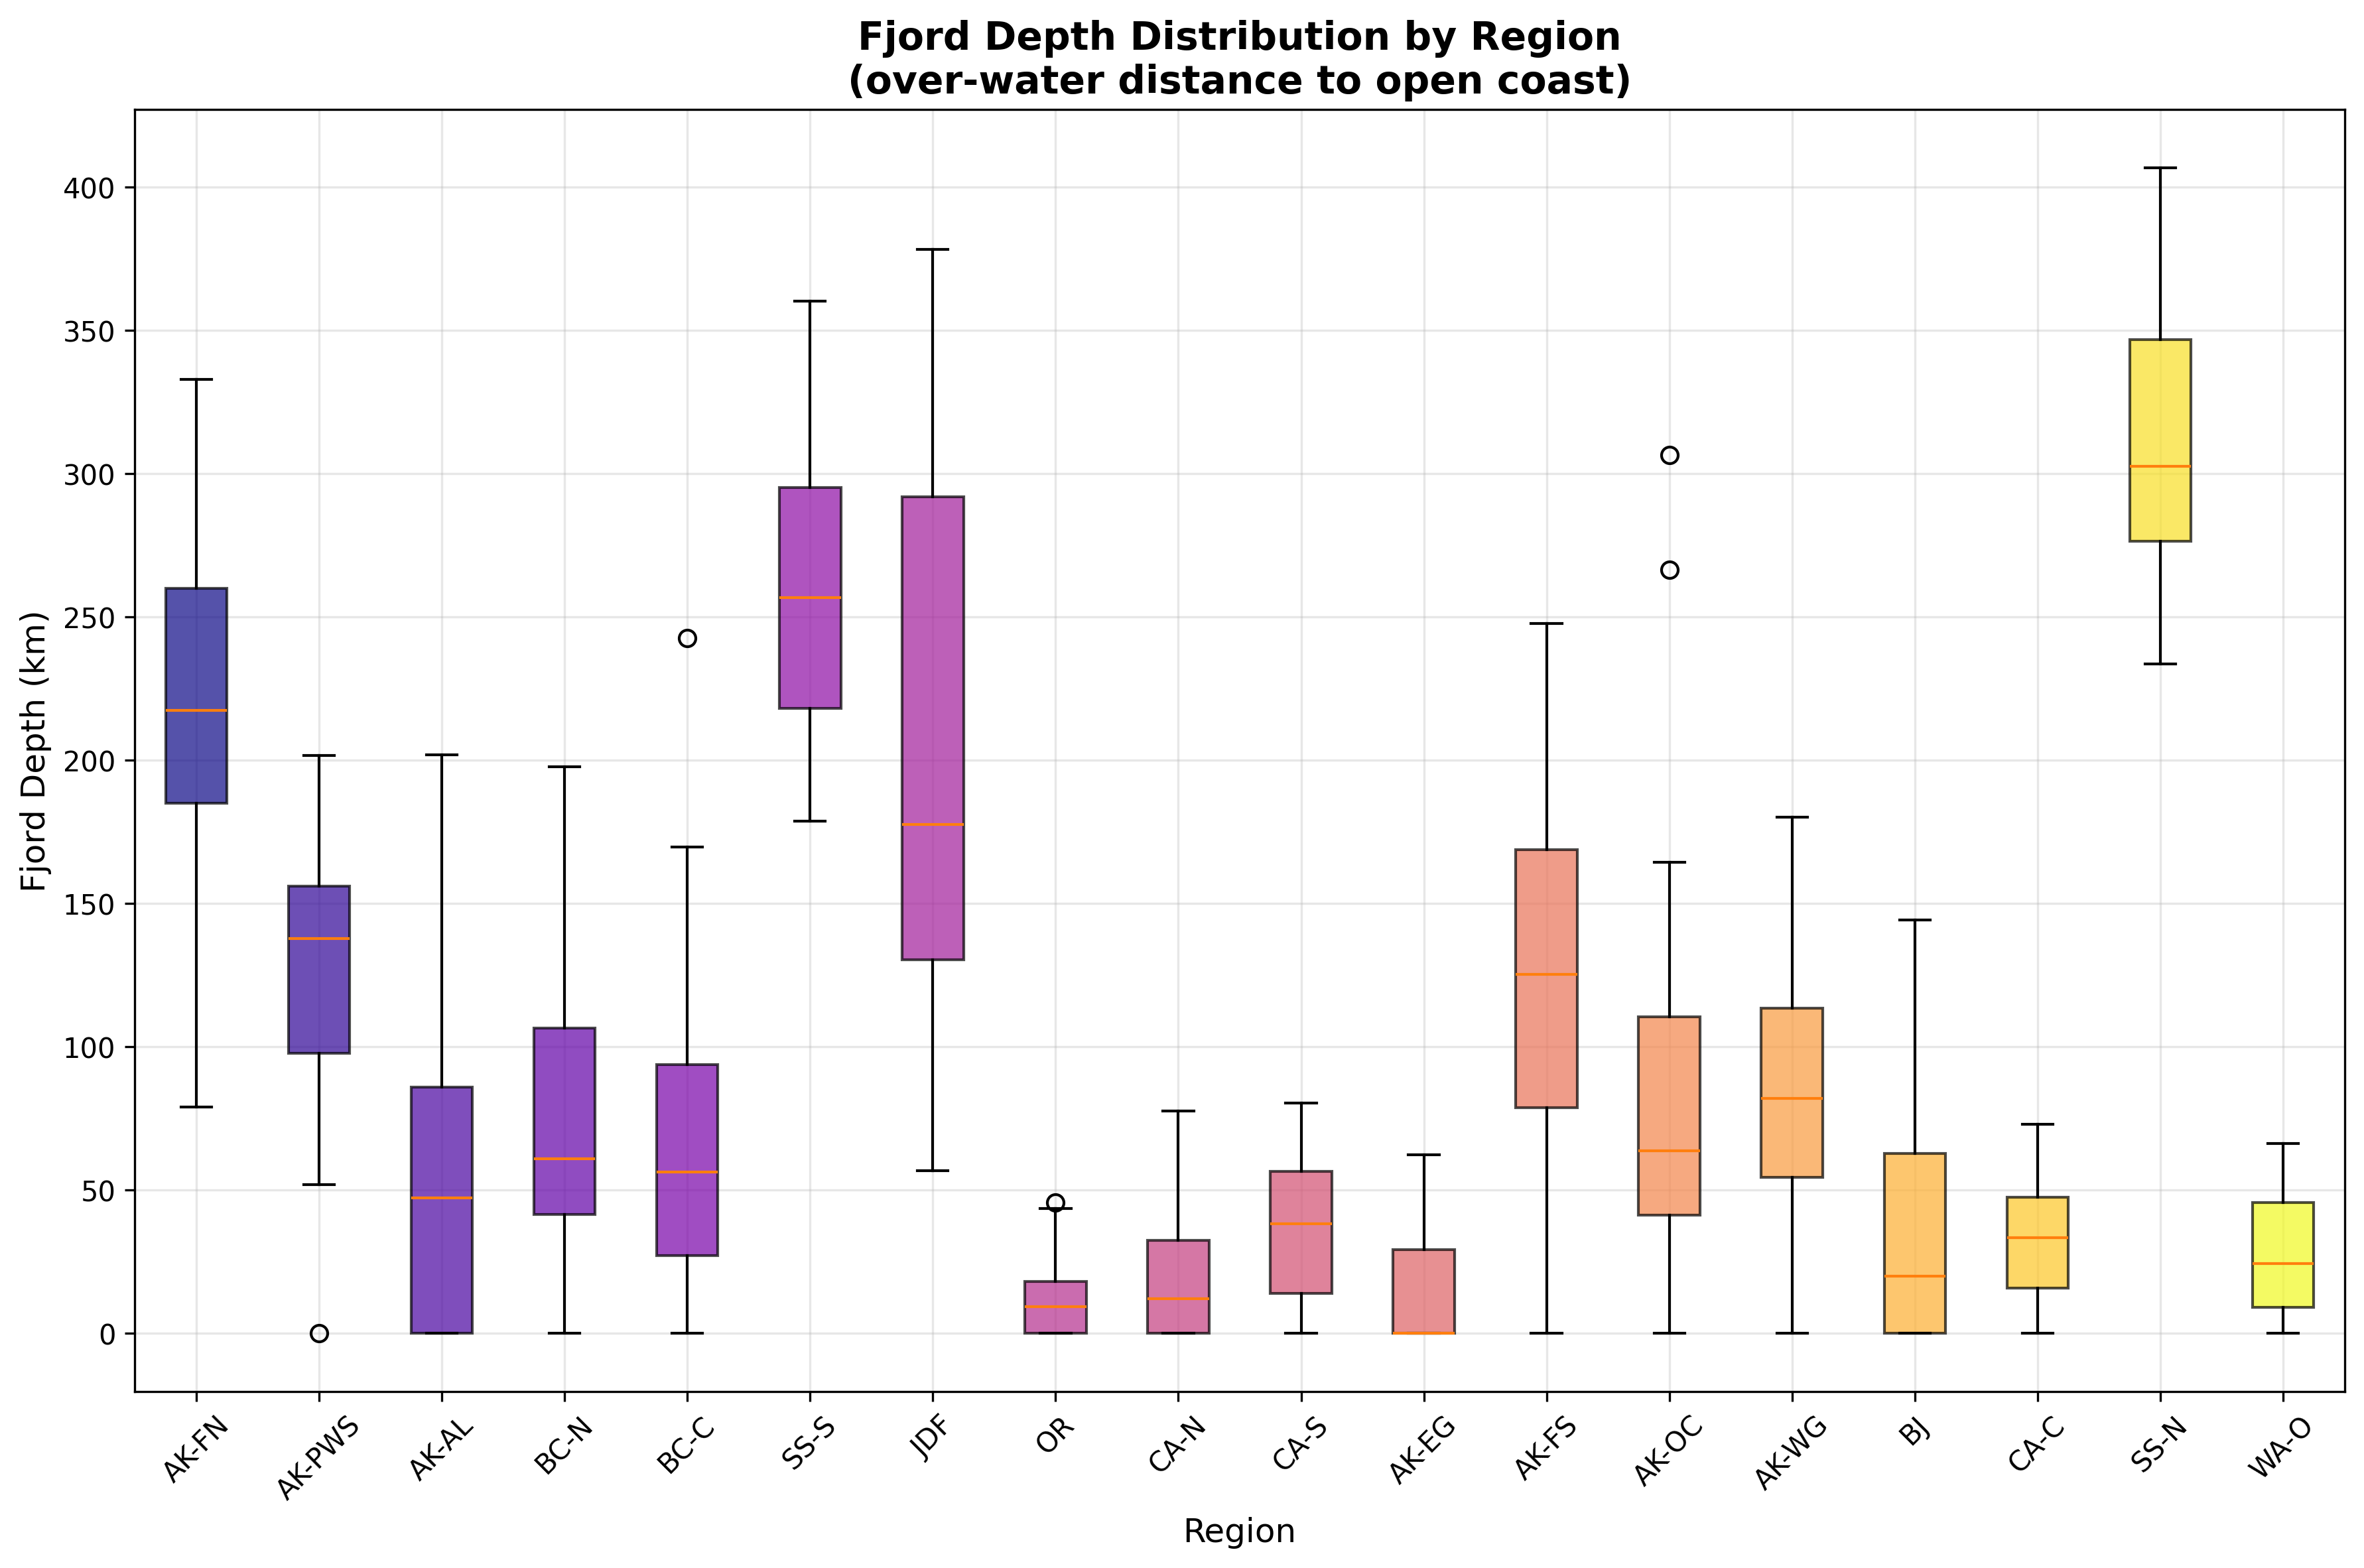
\includegraphics[width=0.95\textwidth]{figures/06_depth_by_region.png}
    \caption{Distribution of fjord depths by region. Puget Sound (SS-S) and Strait of Juan de Fuca (JDF) show exceptional isolation from oceanic water masses, with mean depths exceeding 200 km.}
    \label{fig:depth_regions}
\end{figure}

\subsection{Impact of Fjord Depth Correction}

Figure~\ref{fig:before_after} illustrates the effect of incorporating fjord depth into flushing rate calculations. Points above the 1:1 line indicate sites where fjord depth increased estimated flushing (typically fjord mouths), while points below indicate reduced flushing (fjord heads).

\begin{figure}[H]
    \centering
    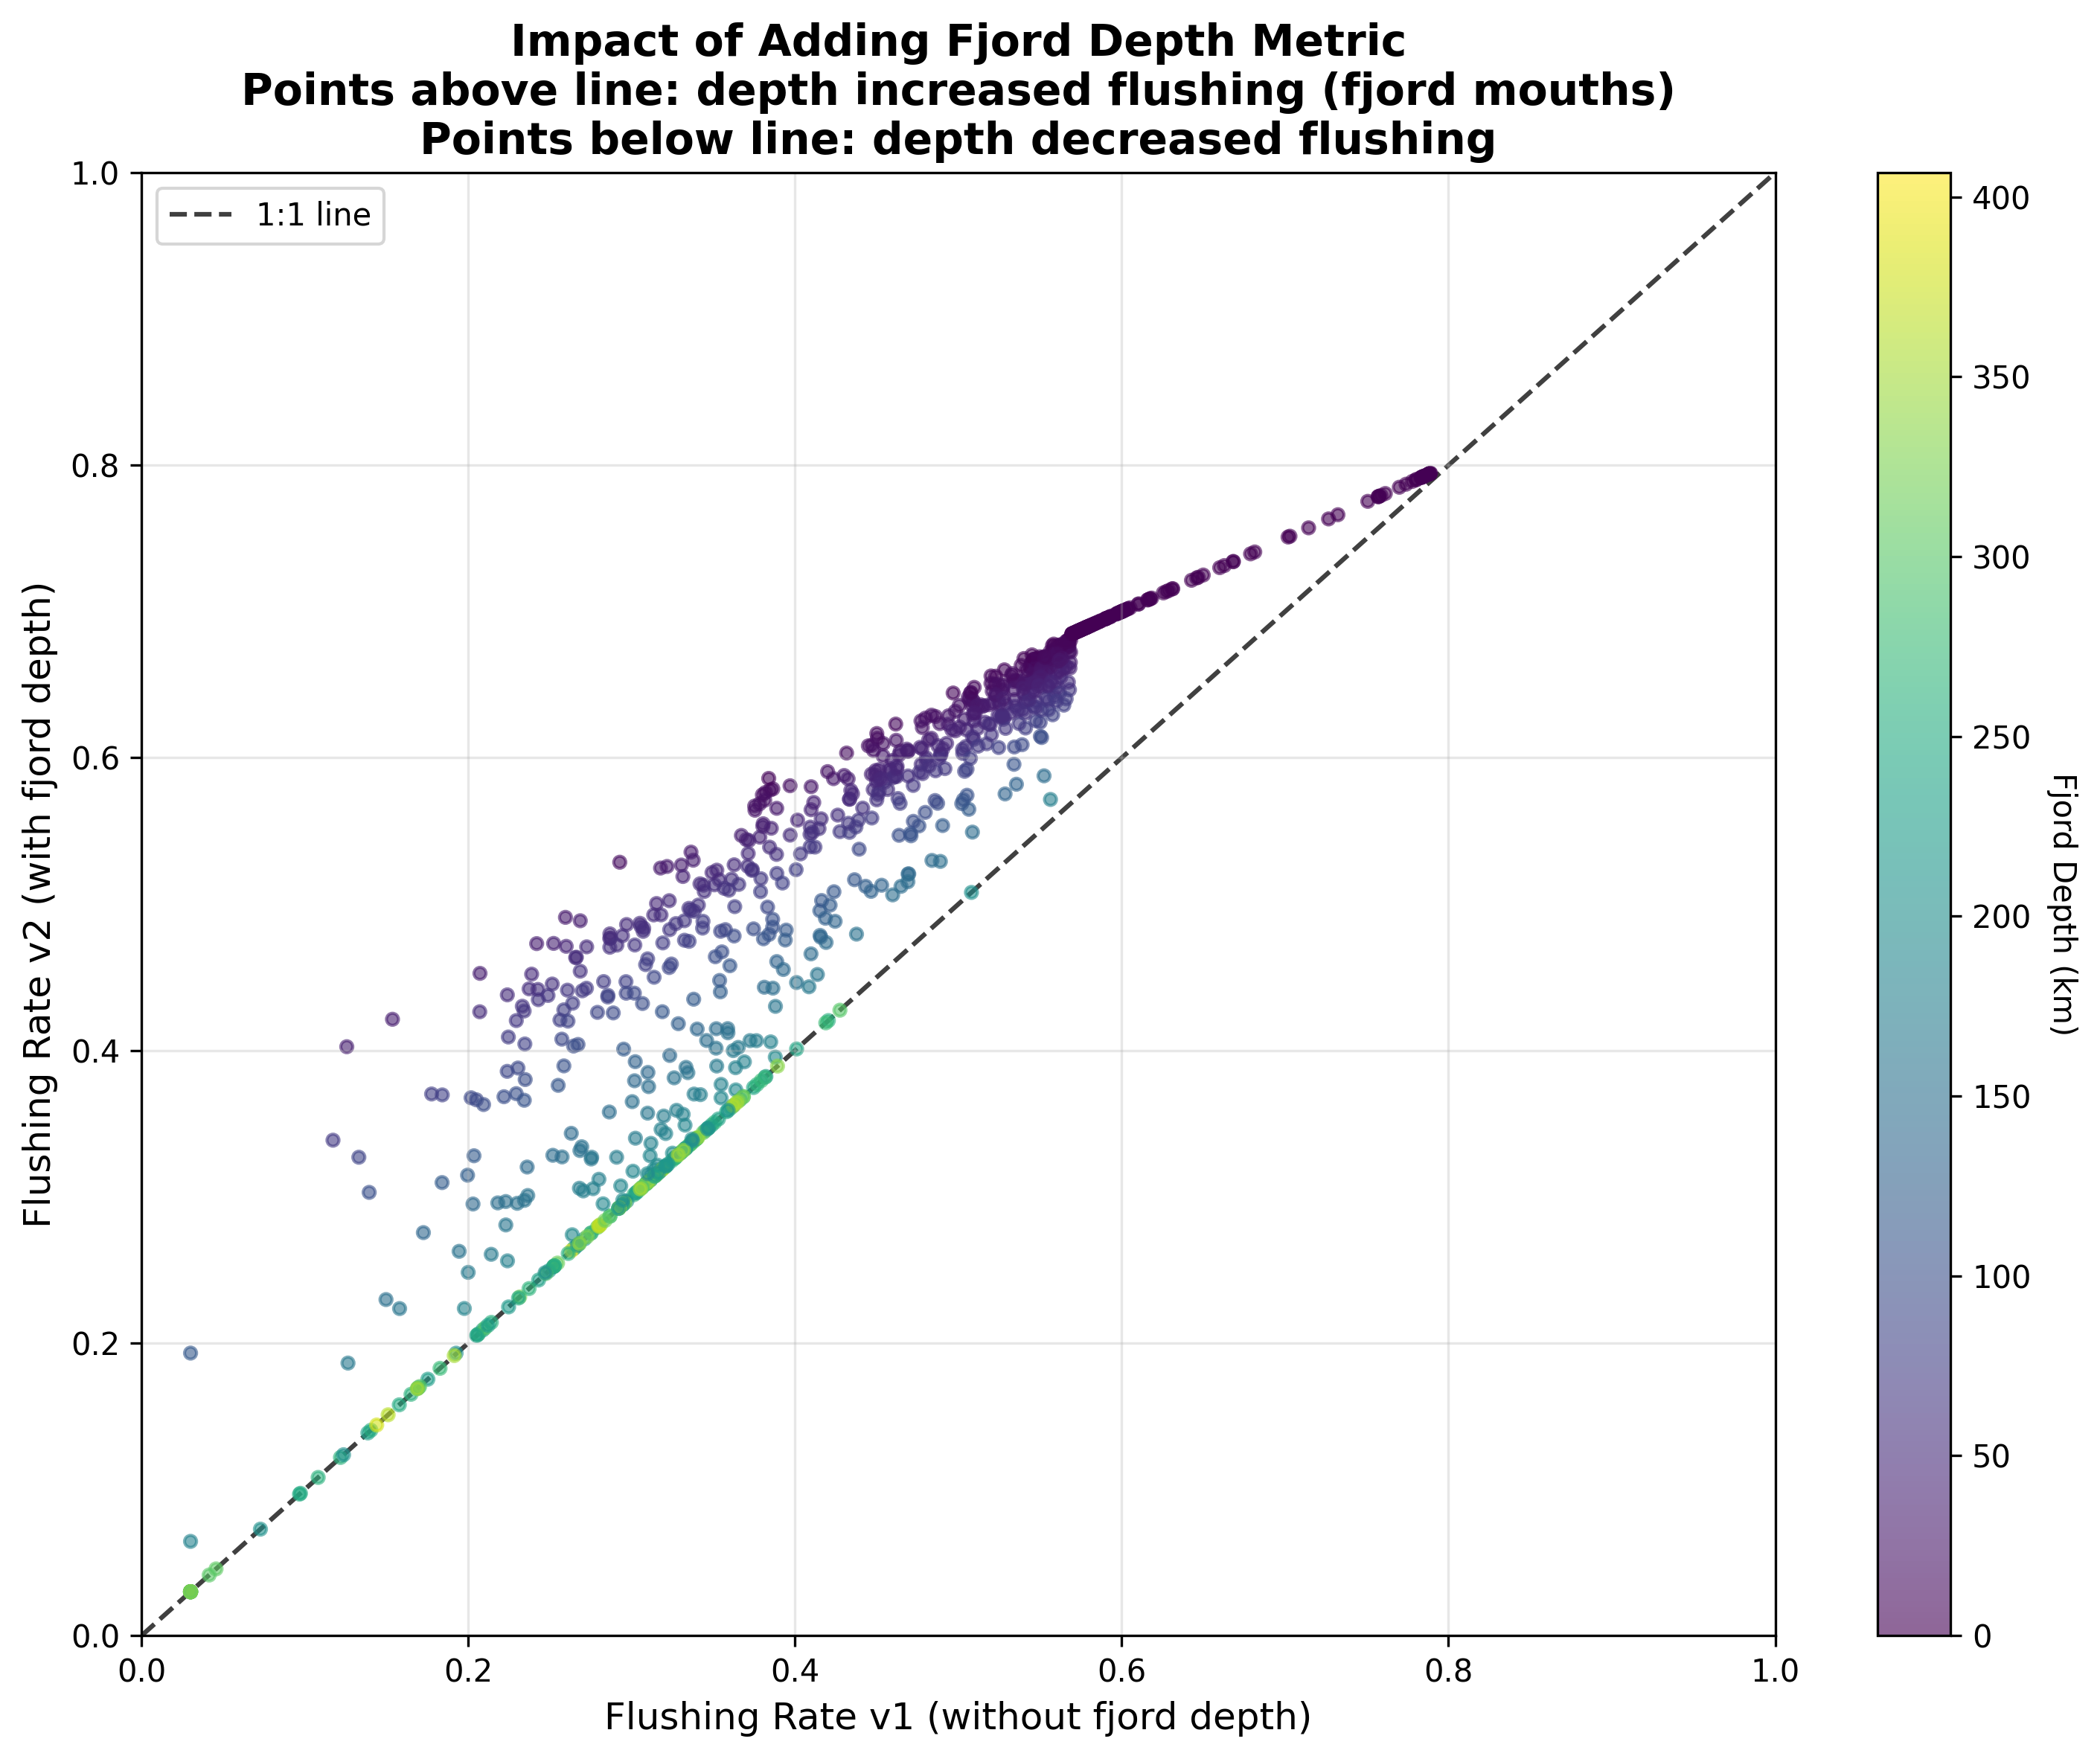
\includegraphics[width=0.9\textwidth]{figures/07_before_after_depth.png}
    \caption{Comparison of flushing rates before (v1) and after (v2) incorporating fjord depth. Points are colored by fjord depth. Sites above the 1:1 line experienced increased flushing estimates (fjord mouths with oceanic access), while sites below experienced decreased estimates (deep fjord sites).}
    \label{fig:before_after}
\end{figure}

\subsection{Regional Summary Statistics}

Figure~\ref{fig:regional_means} summarizes mean flushing rates by region with uncertainty estimates. The north-south gradient is evident, with Alaskan and Puget Sound regions showing low flushing ($\phi < 0.4$) and Pacific coastal regions showing high flushing ($\phi > 0.6$).

\begin{figure}[H]
    \centering
    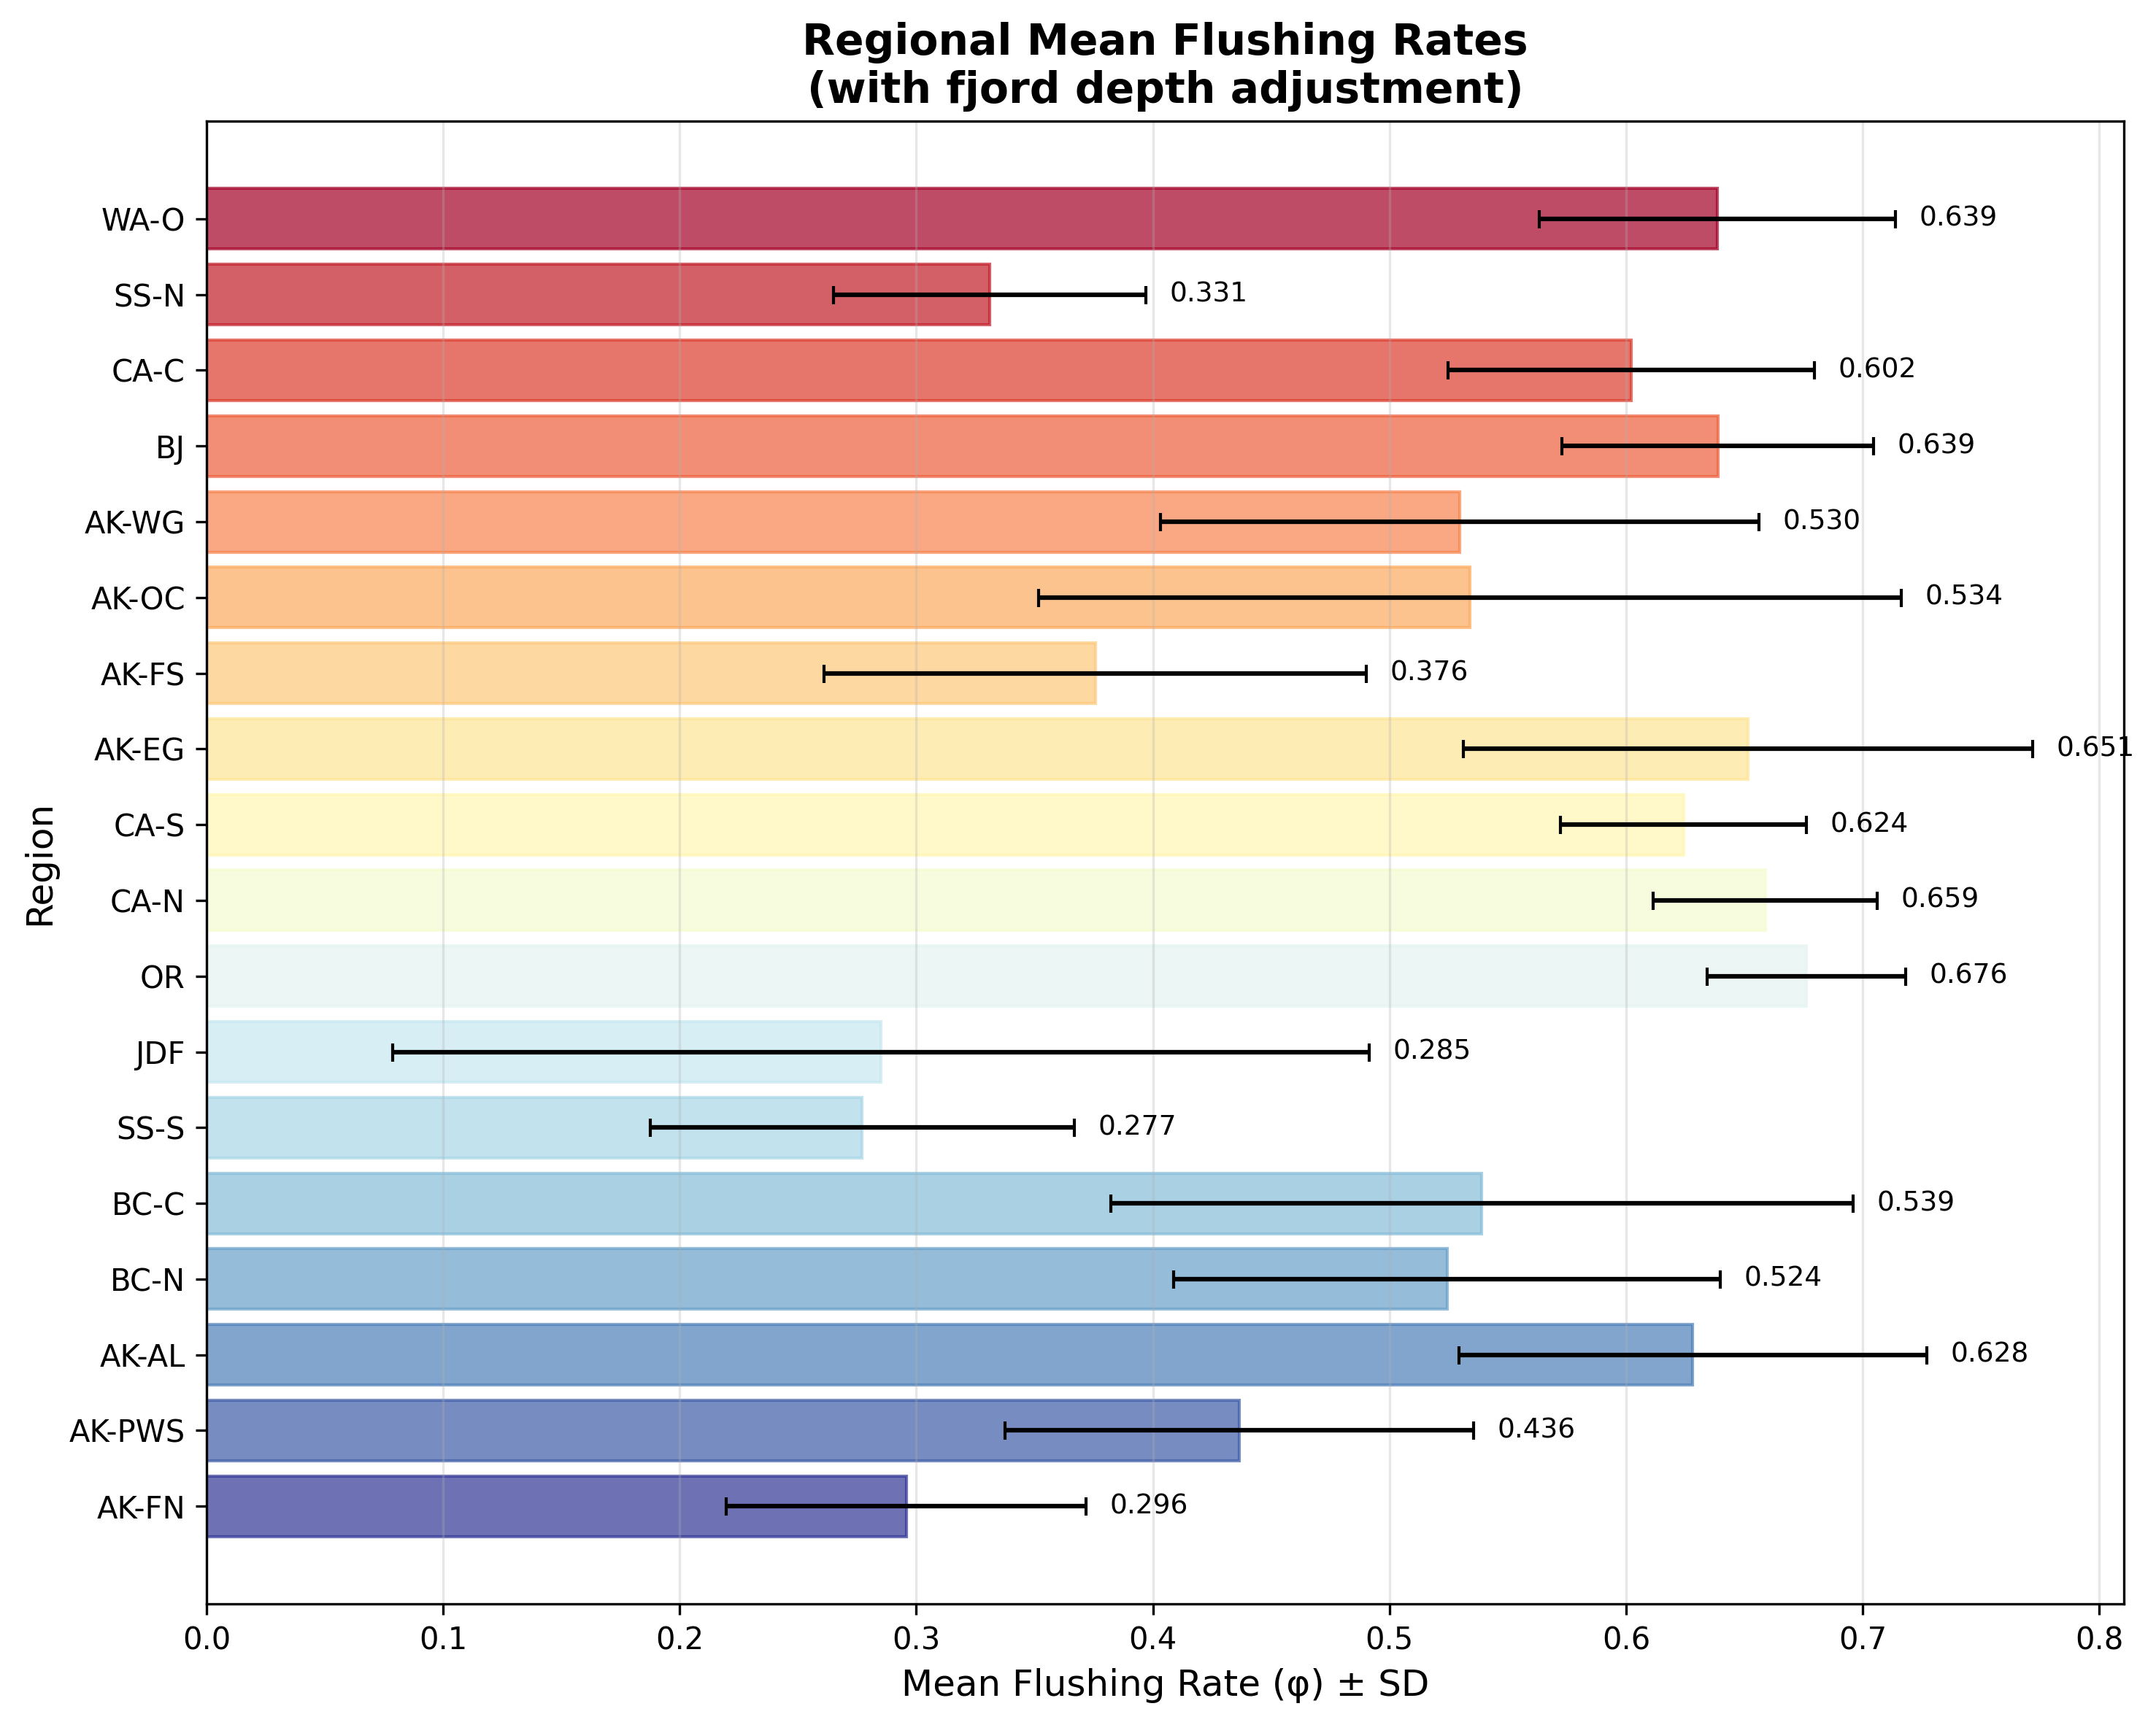
\includegraphics[width=0.95\textwidth]{figures/08_mean_flushing_by_region.png}
    \caption{Regional mean flushing rates with standard deviation error bars. Values are displayed for each region. The clear north-south gradient reflects the transition from complex fjord systems to exposed coastlines.}
    \label{fig:regional_means}
\end{figure}

\section{Key Findings}

\subsection{Successful Waterway Position Discrimination}

The fjord depth metric successfully distinguishes position along waterway systems. Sites deep within the Puget Sound system (SS-S: 259 km) and Strait of Juan de Fuca (JDF: 204 km) are isolated by hundreds of kilometers of over-water distance from oceanic water masses, receiving dramatically reduced flushing rates ($\phi = 0.277$ and $\phi = 0.285$, respectively).

In contrast, exposed Pacific coastal sites in Oregon (11 km mean depth, $\phi = 0.676$) and Northern California (20 km mean depth, $\phi = 0.659$) maintain direct access to oceanic waters with correspondingly high flushing rates.

\subsection{Regional Flushing Hierarchy}

Clear regional patterns emerge:

\begin{itemize}
    \item \textbf{Lowest flushing}: SS-S ($\phi = 0.277$), JDF ($\phi = 0.285$), AK-FN ($\phi = 0.296$)
    \item \textbf{Moderate flushing}: AK-PWS ($\phi = 0.436$), various BC and WA regions
    \item \textbf{Highest flushing}: OR ($\phi = 0.676$), CA-N ($\phi = 0.659$), CA-S ($\phi = 0.624$)
\end{itemize}

\subsection{Dual Effects on Pathogen Dynamics}

The refined flushing estimates reveal critical implications for pathogen transmission modeling:

\subsubsection{During Epidemics}
Low flushing in deep fjords promotes pathogen accumulation through:
\begin{itemize}
    \item Reduced dilution of infectious particles
    \item Extended residence time of waterborne pathogens
    \item Concentration effects in enclosed water masses
\end{itemize}

\subsubsection{During Recovery}
The same isolation that promotes accumulation during epidemics becomes protective during recovery:
\begin{itemize}
    \item Blocked importation of pathogens from infected regions
    \item Accelerated local pathogen decay in isolated water masses
    \item Natural quarantine effects in deep fjord systems
\end{itemize}

This dual effect may explain both the severe crashes observed in enclosed waters during SSWD outbreaks AND the improved recovery potential once local pathogen loads decay.

\section{Biological Significance}

\subsection{Pathogen Transmission Implications}

The spatial structure revealed by this analysis has profound implications for understanding SSWD transmission dynamics:

\textbf{Connectivity Gradients}: The fjord depth metric captures realistic connectivity to oceanic pathogen sources, moving beyond simple geometric enclosedness to incorporate functional isolation.

\textbf{Transmission Barriers}: Deep fjord sites (>200 km depth) effectively represent isolated populations during the critical early phases of outbreaks, when oceanic inoculum drives initial infections.

\textbf{Recovery Sanctuaries}: The same sites that suffer severe impacts during epidemics (due to pathogen accumulation) may serve as recovery sanctuaries once external inoculum is eliminated.

\subsection{Model Parameterization}

These flushing rates provide spatially-explicit parameters for:
\begin{itemize}
    \item Waterborne pathogen transport between sites
    \item Local pathogen persistence vs.\ dilution
    \item Recovery rate modifications based on isolation
    \item Metapopulation source-sink dynamics
\end{itemize}

\section{Discussion}

\subsection{Methodological Advances}

The incorporation of fjord depth represents a significant advance over purely geometric measures of enclosedness. While tortuosity and horizon exposure capture local waterway structure, fjord depth quantifies functional connectivity to oceanic water masses—a critical parameter for understanding pathogen dispersal in marine systems.

\subsection{Validation Against Observations}

The spatial patterns revealed align well with observed SSWD dynamics:
\begin{itemize}
    \item Puget Sound's exceptional isolation (259 km depth) corresponds to observed severe impacts and slow recovery
    \item Oregon's high flushing (11 km depth) aligns with rapid pathogen spread but also rapid recovery
    \item Alaska's heterogeneity (27-219 km depth range) matches variable outbreak patterns across regions
\end{itemize}

\subsection{Future Applications}

This framework extends beyond SSWD to any waterborne marine pathogen system. The three-metric approach provides a generalizable method for characterizing marine connectivity across scales from local embayments to ocean basins.

\section{Conclusions}

This analysis demonstrates the critical importance of incorporating fjord depth into marine connectivity assessments. The resulting flushing rate estimates ($\phi = 0.030$ to $0.795$) reveal previously hidden gradients in pathogen transmission potential across Pacific Northwest marine systems.

Key achievements include:
\begin{itemize}
    \item Development of a novel fjord depth metric capturing functional isolation
    \item Comprehensive analysis of 896 sites across 18 biogeographic regions
    \item Clear demonstration of north-south flushing gradients
    \item Identification of critical transmission barriers and recovery sanctuaries
    \item Spatially-explicit parameterization for epidemic modeling
\end{itemize}

The dual nature of fjord isolation—promoting both pathogen accumulation during outbreaks and pathogen exclusion during recovery—provides a mechanistic explanation for the complex spatiotemporal patterns observed in SSWD dynamics. These insights will prove invaluable for predictive modeling of marine disease transmission and recovery processes.

\section*{Data Availability}

Site enclosedness data including all metrics and derived flushing rates are available in the SSWD-EvoEpi repository at:
\texttt{/data/nodes/site\_enclosedness.json}

Analysis code and figure generation scripts are provided in:
\texttt{/reports/enclosedness\_v2/generate\_report.py}

\end{document}